\label{fs-framework}

Our task is to design a framework for end-to-end text streams multi-classification that overcomes the challenges mentioned above. We assume that there are two types of input stream elements: labeled and unlabeled texts. The framework must use the first ones for additional training. For the others, labels should be predicted and delivered to the user.

\begin{figure}[htbp]
  \centering
  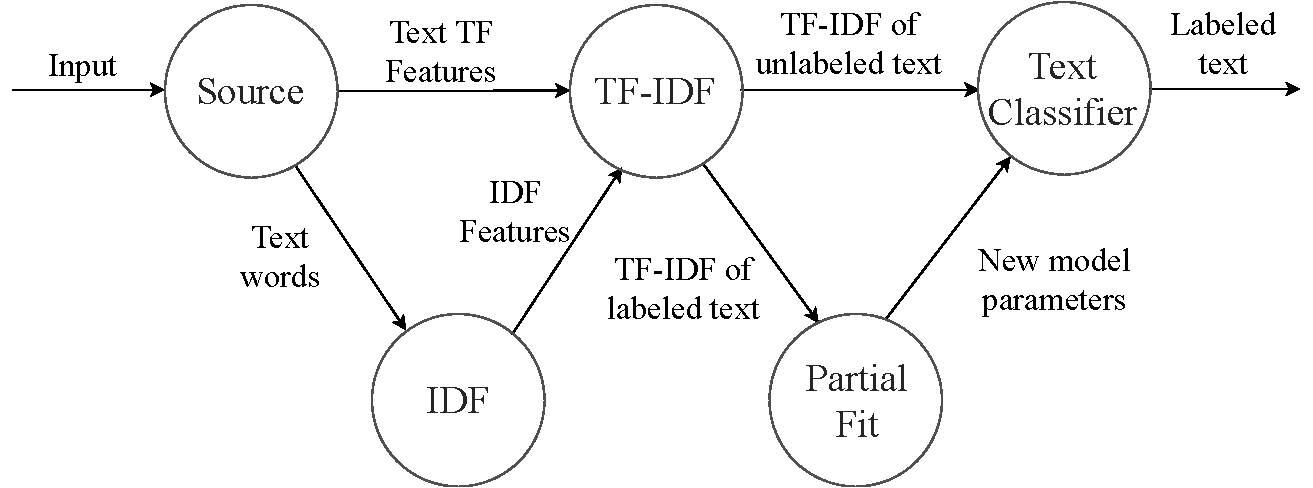
\includegraphics[scale=0.48]{pics/logical-graph}
  \caption{The logical pipeline}
  \label {logical_graph}
\end{figure}

\subsection{Data flow \label{DF}}

\subsubsection{Computational pipeline}

Usually, texts classification consists of the two most important steps. The first is obtaining a documents collection and computing TF-IDF features of it, where TF stands for term frequency and IDF for inverse document frequency. The second is training a classifier on these features.

There is a need for mapping these steps into a stream environment. TF features are straightforward to compute. On the other hand, the IDF calculation is a stateful operation, where text collection updated by each text. The logical directed graph(Figure~\ref{logical_graph}) serves this purpose in the FlameStream. A vertex is an operation with the data, and an edge indicates the flow. Incoming texts enter {\em Input} vertex, which computes TF features and sends them to the next vertex. IDF features calculations based on the current document collection, which is updated by each text. {\em TF-IDF} vertex joins both features together and passes to the {\em Text Classifier}, where a label obtaining occurs.

\begin{figure}[htbp]
  \centering
  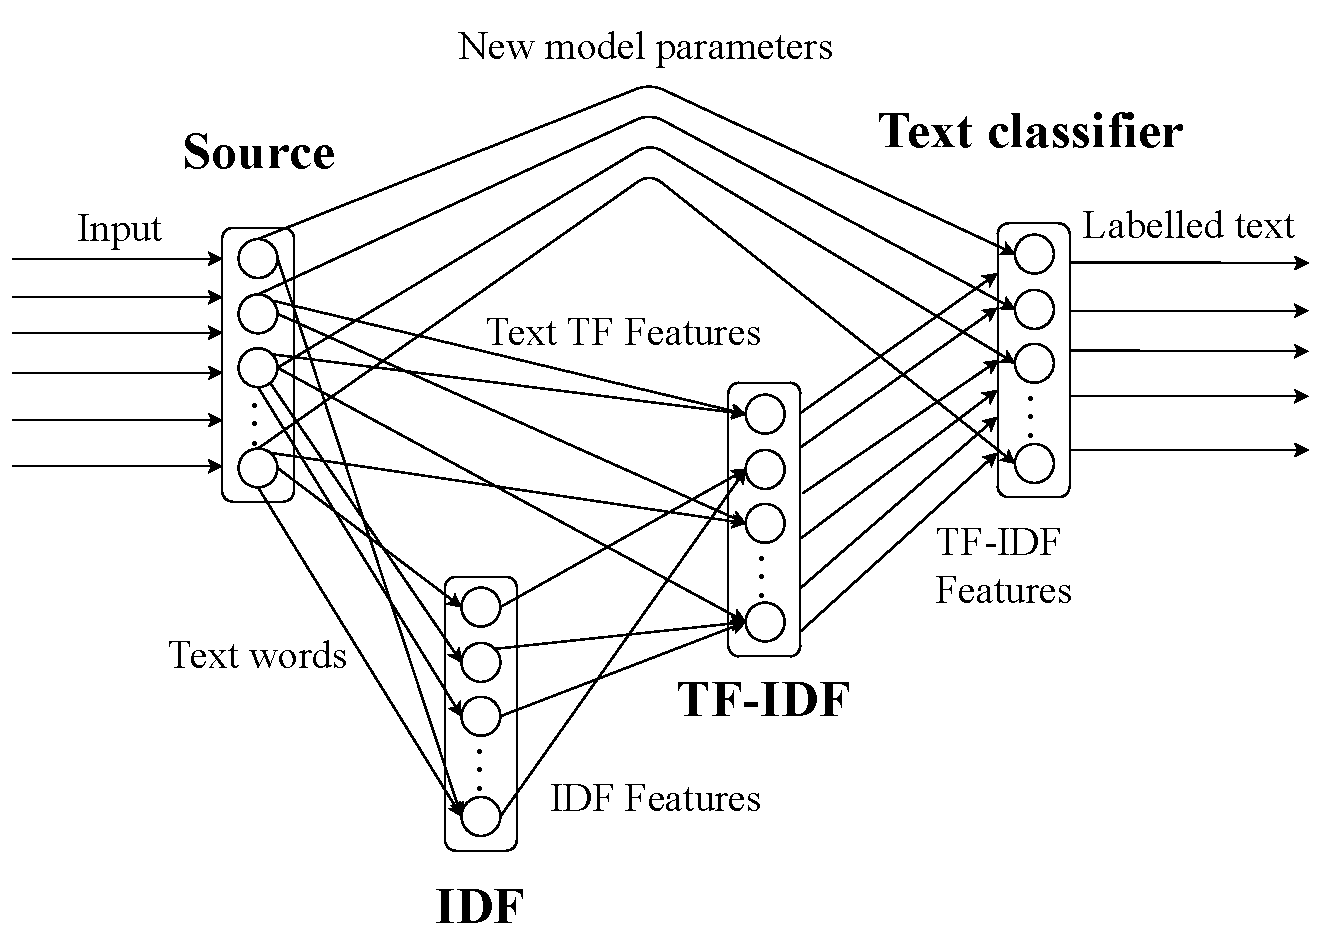
\includegraphics[scale=0.375]{pics/physical-graph}
  \caption{The physical pipeline}
  \label {physical_graph}
\end{figure}

All actual operations executed on all nodes. Scalability is achieved due to data partitioning by keys, which shown in Figure ~\ref{physical_graph}. A node designated by vertex and each rectangle denotes the same cluster. Input before {\em IDF} operation is partitioned by words and before {\em TF-IDF} by text identifier. The classifier executed with the same partitioning as TF-IDF operations. Hence, all operations are scalable. 

\subsubsection{Dealing with concept drift}

Concept drift refers to the particular meaning of words, which changes over time. This aspect may affect the correctness of the pipeline, more specifically, the computing of the IDF features. To overcome the issue, we use windowed IDF calculation: IDF values will be provided based on input within a time window. For instance, the window can be a day or a week. Similar approaches are applied in~\cite{klinkenberg2000detecting}.

\subsubsection{Partial fit}

Figures ~\ref{logical_graph}, ~\ref{physical_graph} provide a scheme for a partial fitting. Partial Fit vertex buffers parts of the stream with labeled text. Additional training is triggered by a special element, which submitted to the Input and every vertex pass this element through to Partial Fit without processing. This process is similar to punctuation~\cite{tucker2003exploiting} handling. The vertex flushes the buffer and updates the parameters of the model. After that, updated parameters are saved for further training and broadcasted to all {\em Text Classifier} vertices.

\subsection{Machine learning model \label{ML}}

The classifier's model can be chosen independently from other computations. In our case, we use Multinomial Logistic Regression. At the start of the system, the initial classifier parameters such as weights can be provided by a pre-train process.

Every time, when the Partial Fit is triggered, the following process occurs, which can be described in terms of the optimization of a cost function. This function in our case is written below:

\begin{center}

$$ J(W) = -\frac{1}{m} \sum \limits_{i = 1}^{m} \sum \limits_{j = 1}^{k} \mathbbm{1}_{\left\{y^{(i)} == j\right\}} \cdot \log \frac{\exp\left({W_{j}^Tx^{(i)}}\right) }{\sum \limits_{l = 1}^{k}  \exp\left({W_{l}^Tx^{(i)}}\right) }$$ 
 $$ +  \lambda_1 ||W||_1 + \lambda_2 ||W - W_{prev}||_2 $$

\end{center} 

The number of points in a new dataset is denoted as $m$. The point with index $i$ showed as $x^{(i)}$. The number of classes is $k$. New weights are designated as $W$. The weights, that computed in the previous step, are $W_{prev}$. At the first time of triggering the process, $W_{prev}$ are the pre-trained weights. 

The formula provides the goal of the training. The first component is the standard softmax function for multiple classes. The second component keeps the l1 regularization of the weights. The important aspect is the regularization provides sparsity, hence, the model has a small size -- about 1 Mb, which can be stored and updated with low cost. To use the previous history of the classifier weights we apply l2 regularization as the third component. Fitting new points and the consideration of the previous weights ensure better accuracy of the classifier.

We are interested in finding such $W$ that minimizes $J(W)$. Taking derivatives, one can show that the gradient for each class component is:

\begin{center}

$$ \nabla_{W_j} \; J(W) = -\frac{1}{m} \sum \limits_{i = 1}^{m} \left[ x^{(i)} \left( \mathbbm{1}_{\left\{y^{(i)} == j\right\} } - \frac{\exp\left({W_{j}^Tx^{(i)}}\right)}{\sum \limits_{l = 1}^{k}  \exp\left({W_{l}^Tx^{(i)}}\right)} \right) \right] $$
$$ - \; \lambda_1 sign\left(W\right) - \frac{\lambda_2}{2} \left(W - W_{prev} \right), \; j = [1..k] $$

\end{center} 

We use Stochastic Gradient Descent for optimization. In experiments ~\ref{fs-short-experiments} section, model performance is presented.